\documentclass[
    11pt, % Set the default font size, options include: 8pt, 9pt, 10pt, 11pt, 12pt, 14pt, 17pt, 20pt
%t, % Uncomment to vertically align all slide content to the top of the slide, rather than the default centered
%aspectratio=169, % Uncomment to set the aspect ratio to a 16:9 ratio which matches the aspect ratio of 1080p and 4K screens and projectors
]{beamer}

\usepackage{booktabs} % Allows the use of \toprule, \midrule and \bottomrule for better rules in tables
\usepackage{xcolor}
\usepackage{listings}
\lstset{
    basicstyle=\ttfamily,
    language=make,
    columns=fullflexible,
    breaklines=true,
    showstringspaces=false,
}
\usepackage{hyperref}

%----------------------------------------------------------------------------------------
% LAYOUT THEME
\usetheme{Madrid}
%----------------------------------------------------------------------------------------

%----------------------------------------------------------------------------------------
% COLOR THEME
\usecolortheme{whale}
%----------------------------------------------------------------------------------------

%----------------------------------------------------------------------------------------
% FONT THEME & FONTS
\usefonttheme{serif}
%----------------------------------------------------------------------------------------

%\usepackage{mathptmx} % Use the Times font for serif text
\usepackage{amsmath}
\usepackage{palatino} % Use the Palatino font for serif text
%\usepackage{helvet} % Use the Helvetica font for sans serif text
\usepackage[default]{opensans}
\usepackage{textcomp} % Use the Open Sans font for sans serif text
\usepackage{scrextend}
%\usepackage[default]{FiraSans} % Use the Fira Sans font for sans serif text
%\usepackage[default]{lato} % Use the Lato font for sans serif text



%----------------------------------------------------------------------------------------
% INNER THEME
\useinnertheme{circles}
%----------------------------------------------------------------------------------------

%\setbeamertemplate{footline} % Removes the footer line in all slides
%\setbeamertemplate{footline}[page number] % Replace the footer line in all slides with a simple slide count
%\setbeamertemplate{navigation symbols}{} % Remove the navigation symbols from the bottom of all slides

%----------------------------------------------------------------------------------------
%	PRESENTATION INFORMATION
\title[microcity]{Micro City - Amusement Park Simulation \\ Intelligent Cyber Physical Systems}
\author[Marcantoni, Romagnoli]{Alessandro Marcantoni\\Simone Romagnoli}
\date[05/08/2022]{05/08/2022}
%----------------------------------------------------------------------------------------

\begin{document}

% TITLE SLIDE ----------------------------------------------------------------------------
    \begin{frame}
        \titlepage
    \end{frame}
%----------------------------------------------------------------------------------------

% TABLE OF CONTENTS SLIDE ---------------------------------------------------------------
    \begin{frame}
        \frametitle{Overview}
        \tableofcontents
    \end{frame}
%----------------------------------------------------------------------------------------

    \section{Introduction}\label{sec:introduction}
\frame{\tableofcontents[currentsection]}

%-------------------------------------------------
\subsection{Domain Context}\label{subsec:domain-context}
\begin{frame}
    \frametitle{Domain Context}
    The concept of \textbf{Micro City} was born observing contexts in which \textit{self-awareness} and \textit{situatedness} might help improve people's experience.

    \bigskip

    We believe that in these contexts wearable devices (and applications running on them) can have a great impact on how people interact with the environment.

\end{frame}
%------------------------------------------------

\subsection{What is a Micro City?}\label{subsec:what-is-a-micro-city?}
\begin{frame}
    \frametitle{What is a Micro City?}
    A \textit{Micro City} is an area with:
    \begin{itemize}
        \item bounded temporal and spatial extension;
        \item various activities in the form of services or events;
        \item people (\textit{guests}) that are interested in these activities and populate the \textit{Micro City} itself because of them;
    \end{itemize}

    \bigskip

    Thus, some examples of \textit{Micro Cities} could be shopping centers, fairs, \textit{amusement parks}, city centers, etc.

\end{frame}
%------------------------------------------------

\subsection{Recommendations}\label{subsec:recommendations}
\begin{frame}
    \frametitle{Recommendations}
    In this context, the introduction of a \textbf{situated recommendation system} could proactively provide recommendations to the guests that, if willing to follow them, would receive rewards.

    \bigskip

    The recommendations could be generated thanks to various policies and the rewards could vary depending on the context of the \textit{Micro City} itself (discounts, cashback, simple reduction of waiting time, etc.)
\end{frame}
%------------------------------------------------

\begin{frame}
    \frametitle{Rewards}
    \begin{columns}
        \begin{column}{0.5\textwidth}
            \begin{addmargin}[0.6em]{2em}
                The following diagram shows the process of obtaining a reward when receiving a recommendation.
            \end{addmargin}
        \end{column}
        \begin{column}{0.5\textwidth}
            \begin{center}
                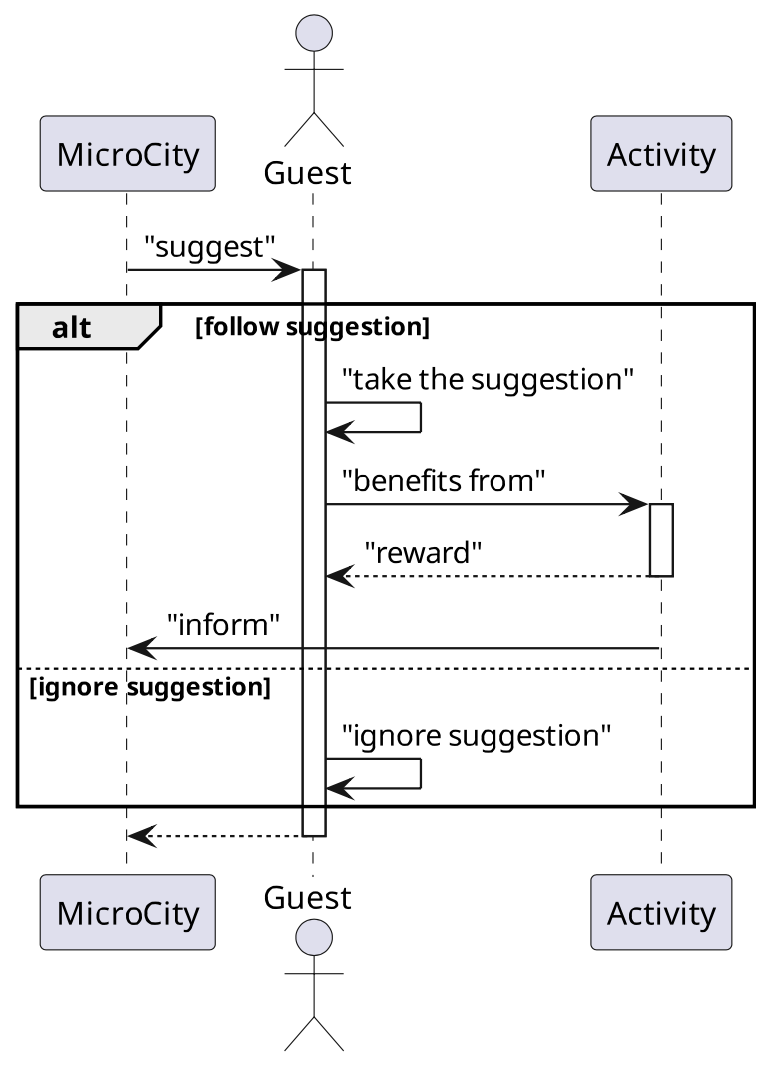
\includegraphics[width=0.9\textwidth]{../img/rewards}
                \label{fig:rewards}
            \end{center}
        \end{column}
    \end{columns}
\end{frame}


    \section{Case Study}\label{sec:case-study}
\frame{\tableofcontents[currentsection]}

%-------------------------------------------------
\subsection{Amusement Park}\label{subsec:amusement-park}

\begin{frame}
    \frametitle{Amusement Park}
    Amusement parks are considered to be a large business all around the world and attract people of every age and culture.

    \bigskip

   They can be considered \textit{Micro Cities} because:
    \begin{itemize}
        \item they develop in a bounded spatial area and are open daily for a given amount of hours;
        \item
    \end{itemize}

\end{frame}
%------------------------------------------------




\end{document}
